%File: datawiseagent_paper.tex
\documentclass[letterpaper]{article} % DO NOT CHANGE THIS
\usepackage[submission]{aaai2027}  % DO NOT CHANGE THIS
\usepackage[hyphens]{url}  % DO NOT CHANGE THIS
\usepackage{graphicx} % DO NOT CHANGE THIS
\urlstyle{rm} % DO NOT CHANGE THIS
\def\UrlFont{\rm}  % DO NOT CHANGE THIS
\usepackage{natbib}  % DO NOT CHANGE THIS AND DO NOT ADD ANY OPTIONS TO IT
\usepackage{caption} % DO NOT CHANGE THIS AND DO NOT ADD ANY OPTIONS TO IT
\frenchspacing  % DO NOT CHANGE THIS
\usepackage{booktabs}
\usepackage{tabularx}
\usepackage{amsmath}
\usepackage{amssymb}
\usepackage{algorithm}
\usepackage{algorithmic}
\graphicspath{{figures/}{./}}
%
\pdfinfo{
/TemplateVersion (2027.1)
}

\setcounter{secnumdepth}{0}

\title{DA-HERO: Scaling Data Science Agents through Harness Intelligence}

\author{
    Anonymous Submission
}

\affiliations{}

\begin{document}

\maketitle

\begin{abstract}
Recent work on data-science agents has primarily pursued capability gains through larger foundation models, longer context windows, and increased test-time search. We study a complementary source of capability: the agent harness governing task interpretation, execution, verification, and repair. We introduce \textbf{DA-HERO} (\textbf{D}ata-\textbf{A}gent \textbf{H}arness for \textbf{E}vidence-Grounded \textbf{R}easoning and \textbf{O}rchestration) and frame \emph{Harness Intelligence} as a controllable scaling dimension for data-science agents. Given an underspecified task, data profile, evaluation metric, and output schema, DA-HERO compiles an executable statistical protocol specifying the prediction target, data characteristics, dependency structure, validation policy, metric semantics, and evidence obligations. Execution proceeds through evidence-carrying artifacts: programmatic validators and budgeted, task-local cross-validation probes assess modeling claims without access to hidden evaluation labels; content-digest-based lineage binds validation evidence to finalized outputs; and verified violations trigger stage-localized repair. Risk-aware orchestration expands search, review, and verification in proportion to downstream risk. On InfiAgentBench, DA-HERO improves Accuracy by Question (ABQ) by 8.2 and 12.3 percentage points on the Medium and Hard subsets, respectively. Across model families and scales, DA-HERO consistently translates harness improvements into predictive gains, with especially large gains emerging on compact backbones. On the DataModeling split of DSBench, enhanced harnessing raises the normalized performance of Qwen3-VL-8B from 0.2873 under the reproduced baseline setting to 0.4825 under a common evaluation protocol, closing 79.8\% of the performance gap to Qwen3.5-35B-A3B, which achieves 0.5318. The result shows that Harness Intelligence does not merely prevent malformed or incomplete outputs: it substantially expands the predictive capability attainable from a fixed, compact model. A supplementary controlled same-model ablation on DeepSeek-v4-Flash corroborates this mechanism, improving mean benchmark-normalized performance by 14.8\% across 43 data-accessible tasks under failure-as-zero scoring. Finally, risk-stratified mixed-model execution further reduces pricing-normalized token cost by 41.0\% while retaining 95.9\% of the accuracy achieved by the all-32B configuration. Together, these results establish Harness Intelligence as a model-agnostic mechanism for scaling the predictive capability, reliability, and efficiency of data-science agents.
\end{abstract}

\section{Introduction}

The recent trajectory of LLM agents has inherited a model-centric theory of progress: stronger systems are expected to follow from a larger backbone, a longer context window, or more test-time search. This strategy has produced increasingly capable notebook agents that can plan, write code, execute analyses, and recover from runtime errors~\cite{wang2024data, guo2024data}. Yet a data-science agent is not merely a language model with access to Python. It is a compound decision system whose conclusions depend on whether statistical intent is preserved across task interpretation, data transformation, validation, model selection, and artifact finalization. Scaling the model improves the reasoning substrate; it does not, by itself, specify the scientific process in which that reasoning must operate.

This distinction becomes consequential because an executable analysis is not necessarily a valid one. A random split can inflate performance when patients, users, queries, or timestamps induce dependence. Target encoding can silently leak labels. A classifier can optimize the wrong metric by emitting hard labels where calibrated probabilities are required. A submission can satisfy every CSV constraint while collapsing to a constant prediction. Even a legitimate validation score can become stale when a later repair changes the finalized artifact. These are not isolated code-generation failures. They are failures to preserve the semantics, evidence, and provenance of an analytical decision across an extended trajectory.

We therefore introduce \emph{Harness Intelligence}: the task knowledge, statistical discipline, evidence structures, verification mechanisms, repair policies, and compute-allocation rules externalized around a foundation model. Harness Intelligence is not a guardrail applied after generation. It is an active source of capability that determines which problem the model solves, which evidence it must produce, which claims the system may accept, and where additional reasoning is worth its cost. Model intelligence supplies flexible hypothesis generation and program synthesis; harness intelligence turns those capabilities into a controlled scientific process. This view makes the model--harness pair, rather than the model alone, the relevant unit of agent design and evaluation.

We instantiate this view in \textbf{DA-HERO}: the \textbf{D}ata-\textbf{A}gent \textbf{H}arness for \textbf{E}vidence-Grounded \textbf{R}easoning and \textbf{O}rchestration. Rather than asking one model trajectory to internalize an entire data scientist, DA-HERO compiles data-science discipline into an executable architecture around the model. A protocol compiler derives an orthogonal task signature from the prediction target, data modality, dependency structure, split constraints, metric semantics, submission schema, and resource conditions. It then instantiates a stage graph with task-specific operators and explicit evidence obligations. The same foundation model can consequently behave differently when confronting grouped classification, temporal regression, unstructured text, or a closed-form statistical query---not because the prompt contains a longer generic checklist, but because the harness changes the admissible analytical protocol.

DA-HERO executes this protocol through \emph{evidence-carrying state}. Data profiles, answer specifications, stage reports, validation summaries, verifier findings, and finalized outputs are represented as compact typed artifacts instead of being buried in a growing notebook transcript. Programmatic checks corroborate claims that should not depend on model judgment; public-data proxy experiments test whether candidate modeling choices improve over defensible baselines; and content digests bind validation evidence to the artifact that is ultimately submitted. When a constraint is violated, the system converts the verified failure into a stage-localized repair plan. This transforms retry from wholesale regeneration into targeted self-correction, limiting both context contamination and the risk of damaging already-valid work. Specialized stage agents serve as cognitive operators within this protocol, while a role-separated review agent interrogates high-risk decisions without duplicating the entire execution history.

Harness Intelligence also changes how inference should be budgeted. Uniformly assigning a frontier model to profiling, schema checks, formatting, diagnosis, and modeling treats all tokens as equally valuable and all errors as equally costly. DA-HERO instead allocates reasoning according to downstream risk: deterministic programs handle invariant checks, compact models or bounded calls handle low-risk interpretation, and stronger reasoning, review, or repair is activated where a mistake can invalidate the scientific result. We operationalize this trade-off with EqTok, a pricing-normalized measure for heterogeneous model execution.

We evaluate DA-HERO in two complementary regimes. \textbf{InfiAgentBench} contains 257 closed-form data-analysis questions across ABQ, PASQ, and UASQ settings, testing exact analytical correctness and answer rendering~\cite{infiagentbench}. \textbf{DataModeling} contains 74 Kaggle-style predictive tasks~\cite{kaggle}; 43 tasks with accessible datasets support a controlled same-model comparison. Protocolized execution improves Medium and Hard ABQ accuracy by 8.2 and 12.3 percentage points. On the 43 DataModeling tasks, DA-HERO increases scoreable completion from 90.7\% to 100\% and strict mean normalized performance by 14.8\% relative to the model-only baseline. Restricting the comparison to the 39 tasks completed by both systems preserves an 8.5\% relative gain, showing that the improvement is not explained solely by recovering failed runs. A mixed-model configuration reduces EqTok by roughly 40\% while retaining 96\% of reference accuracy.

We make four contributions:

\begin{itemize}
    \item \textbf{Harness Intelligence as a scaling axis.} We formulate a model--harness view of data-science agents in which capability is expanded by externalizing statistical protocols, evidence requirements, verification, repair, and adaptive computation rather than relying only on larger model capacity.
    \item \textbf{Data-science protocol compilation (Section~\ref{sec:task}).} We map task semantics and dataset structure into executable, task-specific protocols over validation, feature construction, modeling, and output obligations, replacing the classification-versus-regression shortcut with a richer decision representation.
    \item \textbf{Evidence-grounded orchestration (Section~\ref{sec:structured}).} We connect typed intermediate artifacts, programmatic corroboration, public-data proxy evaluation, digest-bound lineage, role-separated review, and failure-localized repair into a closed execution loop. To our knowledge, DA-HERO is the first data-science agent architecture to combine these mechanisms as one evidence-preserving protocol.
    \item \textbf{Cross-regime empirical validation (Sections~\ref{sec:resource} and~\ref{sec:discussion}).} We show that the same harness improves exact analysis, scoreable completion, and predictive performance, while risk-stratified inference reduces equivalent-token cost. Same-model comparisons separate genuine modeling gains from structural failure recovery.
\end{itemize}

Harness Intelligence constitutes an independent axis along which agent capability can scale. DA-HERO transforms the harness from passive infrastructure into an executable form of data-science intelligence---one that makes smaller models more disciplined, stronger models more effective, and every finalized result more tightly coupled to the evidence that justifies it.

\section{Related Work}

\subsection{LLM Agents for Data Science}

Recent systems demonstrate that LLMs can serve as the reasoning core of data-science automation.  Frameworks such as OpenHands~\cite{wang2024data} and Data Interpreter~\cite{guo2024data} embed models in execution environments that support planning, code generation, tool use, and iterative debugging.  AutoGen~\cite{wu2023autogen} broadens the design space with multi-agent conversation patterns, while InfiAgentBench~\cite{infiagentbench} provides a benchmark suite for answer-book, partially assisted, and unassisted data-analysis questions.  These systems establish that LLM agents can execute nontrivial analytical workflows.  Our focus is orthogonal: we study how the surrounding runtime should govern task interpretation, evidence flow, and resource allocation when the same agent must handle heterogeneous task regimes.

\subsection{Harness Design and Structured Reasoning}

The behavior of an LLM agent is shaped not only by the base model, but by the harness that specifies constraints, intermediate representations, validators, and output contracts~\cite{white2023prompt}.  Prior work explores chain-of-thought prompting~\cite{wei2022chain}, tree-of-thought search~\cite{yao2023tree}, self-consistency~\cite{wang2022self}, structured output parsing~\cite{zheng2023judgelm}, and constraint-oriented decoding~\cite{lu2024chameleon}.  Much of this literature treats structure as a reasoning aid applied broadly across tasks.  DA-HERO instead treats harness configuration as a routing problem: summary statistics, correlation, machine learning, and predictive modeling require different protocols because they fail in different ways.  The harness is therefore not a single prompt template, but a governed set of contracts selected by task semantics and risk.

\subsection{Resource-Efficient LLM Deployment}

The cost of deploying LLM agents has motivated model cascades~\cite{varshney2022model}, speculative decoding~\cite{leviathan2023fast}, mixture-of-agents architectures~\cite{wang2024mixture}, and task routers that assign queries to models of different sizes~\cite{chen2024fusellm, ong2024route}.  Agent pipelines make the resource problem sharper: a single user task can trigger profiling, planning, code generation, execution, debugging, verification, and formatting.  Counting API calls or raw tokens is insufficient when these stages use heterogeneous models.  EqTok contributes a simple pricing-normalized unit that lets us reason about full-pipeline cost under mixed-model execution.

\subsection{Memory and Context Management}

Long-context models make it tempting to preserve entire interaction histories, yet retrieval and attention quality can degrade as contexts grow~\cite{liu2024lost}.  Memory systems such as MemGPT~\cite{packer2023memgpt} introduce more explicit storage and retrieval policies.  Our contribution is a lightweight alternative specialized to data-science agents: communicate through compact artifacts rather than full transcripts.  DataCards, Answer Specs, and Verifier reports act as typed memory objects that preserve what the next stage needs while excluding stale variables, debug traces, and failed hypotheses.

\section{Problem Setting: Governed Data Science Automation}
\label{sec:background}

\subsection{System Architecture}

DA-HERO builds on DatawiseAgent and organizes data-science automation into three layers.  The \textbf{Agent Core} is a notebook-oriented finite-state transducer with four states: planning, execution, debugging, and post-debug filtering.  It generates Python cells, executes them, diagnoses failures, and retains the working path.  In the default baseline, the same model is used across these stages regardless of whether the current operation is high-risk reasoning or deterministic bookkeeping.

The \textbf{Governance Layer} is the main object of this paper.  It contains deterministic and structured modules that wrap the agent core: DataCard for schema profiling, Contract for answer specification, Skill Checklist for required operations, Oracle and Verifier for semantic and structural checking, Final Block for deterministic answer rendering, Memory and Search for interaction control, Recovery for failure handling, and Rules for reusable constraints.  These modules are deliberately not all LLM calls.  Many are programmatic transformations, validators, or template renderers whose purpose is to make the model's degrees of freedom explicit.

The \textbf{Evaluation Layer} executes benchmarks, reformats outputs, scores closed-form answers, validates modeling submissions, and aggregates metrics.  It supports ablations that enable or disable harness modules, allowing us to measure not merely whether a stronger model helps, but which governance mechanisms change the agent's behavior.

Our experiments use Qwen model variants (8B, 14B, 32B, and 35B-A3B MoE) deployed via API.  Qwen3.5-35B-A3B serves as the strong reference, while Qwen3.5-Flash and smaller Qwen variants stress-test whether structured governance can recover performance from weaker models.

\subsection{Benchmark Profiles}

\textbf{InfiAgentBench (DA-Dev)} comprises 257 data-analysis questions with a balanced difficulty profile: Easy (82, 31.9\%), Medium (87, 33.9\%), and Hard (88, 34.2\%).  Questions are annotated by data-science concept: Summary Statistics (90), Correlation (58), Feature Engineering (37), Machine Learning (19), and Comprehensive Preprocessing (45).  A substantial fraction, 107/257 (41.6\%), involve multiple concepts; these dual-concept questions are markedly harder than single-concept ones (79.4\% vs. 90.7\% baseline accuracy).  The benchmark spans ABQ, PASQ, and UASQ sub-tasks and is scored by exact-match question accuracy (Q-Acc).

\textbf{DataModeling} comprises 74 Kaggle-style predictive modeling tasks.  Here the final object is not a scalar answer but a scoreable CSV submission plus a manifest describing modeling choices.  Evaluation tracks completion rate and normalized predictive performance over task-specific metrics such as AUC, RMSE, and log loss.  The Qwen2.5 baseline completes 68/74 tasks with a normalized performance score of 0.4290 and an average runtime of 760.3 seconds per task.

\begin{figure}[t]
\centering
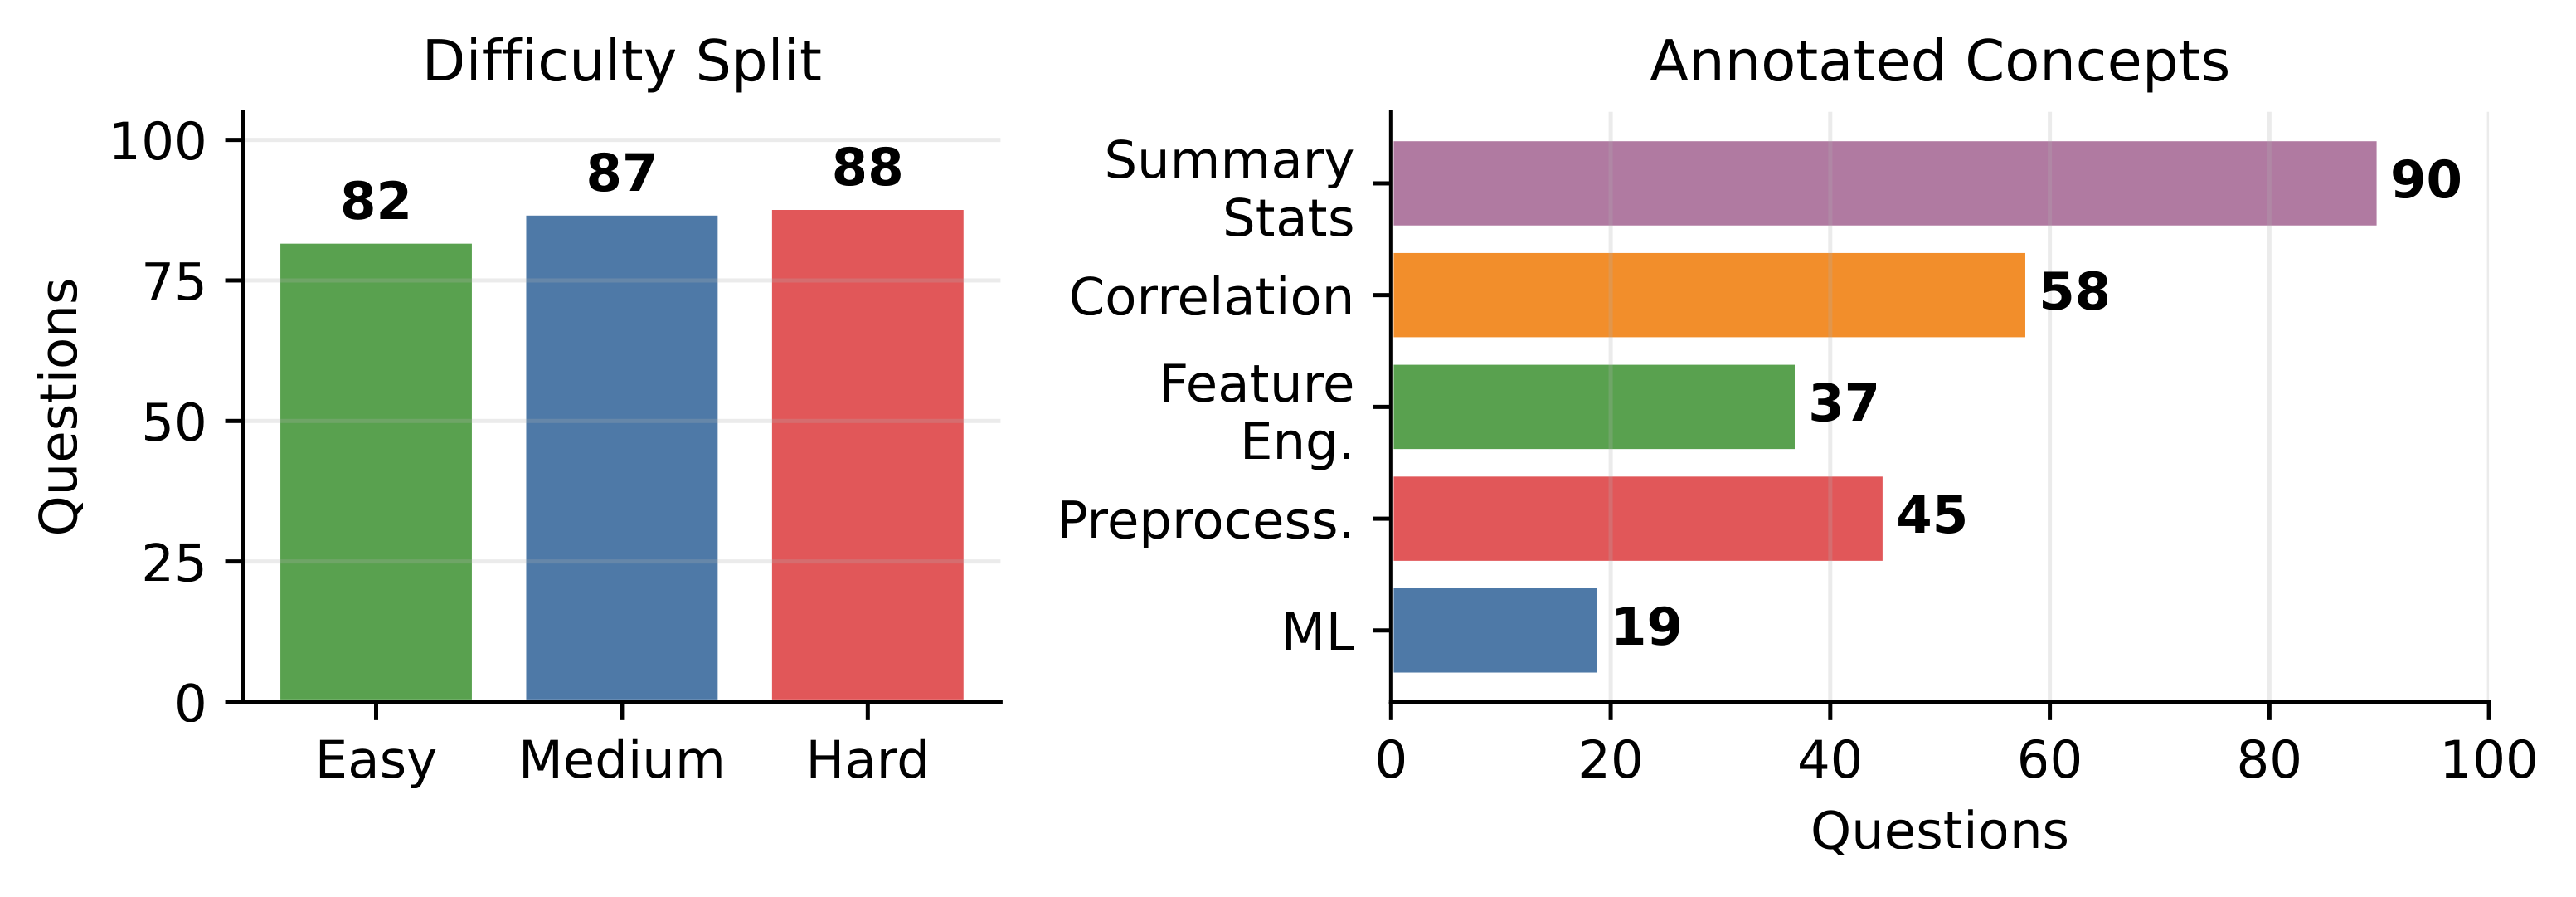
\includegraphics[width=\columnwidth]{task_profile.png}
\caption{InfiAgentBench profile used in our analysis.  Difficulty is approximately balanced, while concept annotations concentrate in summary statistics, correlation, preprocessing, feature engineering, and machine learning.}
\label{fig:task_profile}
\end{figure}

\subsection{Failure Mode Taxonomy}

The two benchmarks expose distinct failure geometries.  \textbf{InfiAgentBench failures} often occur after the agent has done much of the computation correctly: answer-name drift assigns the right value to the wrong key; statistical definition drift changes filters, grouping variables, correlation methods, or rounding rules; and format degradation renders the value as a DataFrame, Series, or explanatory sentence rather than as the required scalar.

\textbf{DataModeling failures} are less about parsing and more about scientific substance.  A submission can be structurally valid while carrying little predictive information: constant regression outputs, single-class classification collapse, uncalibrated probability columns, or a manifest that does not justify why the final file improves over a fallback.  These failures motivate a stronger notion of correctness: a data-science agent should produce not only an accepted artifact, but an artifact supported by task-appropriate evidence.

\begin{table}[t]
\centering
\caption{Baseline performance on InfiAgentBench. Qwen3.5-35B-A3B serves as the strong reference. Qwen3-32B provides a comparable single-model baseline.}
\label{tab:baseline}
\begin{tabular}{lccc}
\toprule
\textbf{Setting} & \textbf{ABQ} & \textbf{PASQ} & \textbf{UASQ} \\
\midrule
Qwen3-32B (full) & 81.74\% & 86.21\% & 86.43\% \\
Qwen3.5-35B-A3B & 86.38\% & 90.16\% & 90.35\% \\
\bottomrule
\end{tabular}
\end{table}

The taxonomy leads to our design thesis: reliability is not a scalar property of the model.  It is a property of the model-runtime pair, and the runtime must govern task semantics, evidence flow, and cost.

\section{Task-Specific Adaptation via Protocol Routing}
\label{sec:task}

\subsection{Task Router Design}

The central design principle of DA-HERO is to classify before constraining.  A summary-statistics question should be governed like a precise mathematical query; a correlation question should declare the method before computation; a machine-learning question should expose validation and model choice; a predictive modeling task should satisfy a submission contract and demonstrate non-degenerate predictive signal.  Uniform prompts either under-constrain tasks that need strict numerical discipline or over-constrain tasks that need modeling flexibility.

Figure~\ref{fig:da_hero_overview} summarizes this control-plane view.  The Harness Orchestrator first maps each benchmark task and dataset into a requirement specification; Part I routes the task through a Task-analyze Agent, Router--Planner, and Skill/MCP Runner; Part II executes, verifies, finalizes, and repairs notebook outputs; Part III supplies memory filtering and resource-risk scheduling.  The router classifies each question along four axes: difficulty, data-science concept, intent keywords, and expected output format.  These axes determine a \textbf{Harness Spec}, a protocol card containing an Answer Spec, Skill Checklist, and Output Contract.

\begin{figure*}[t]
\centering
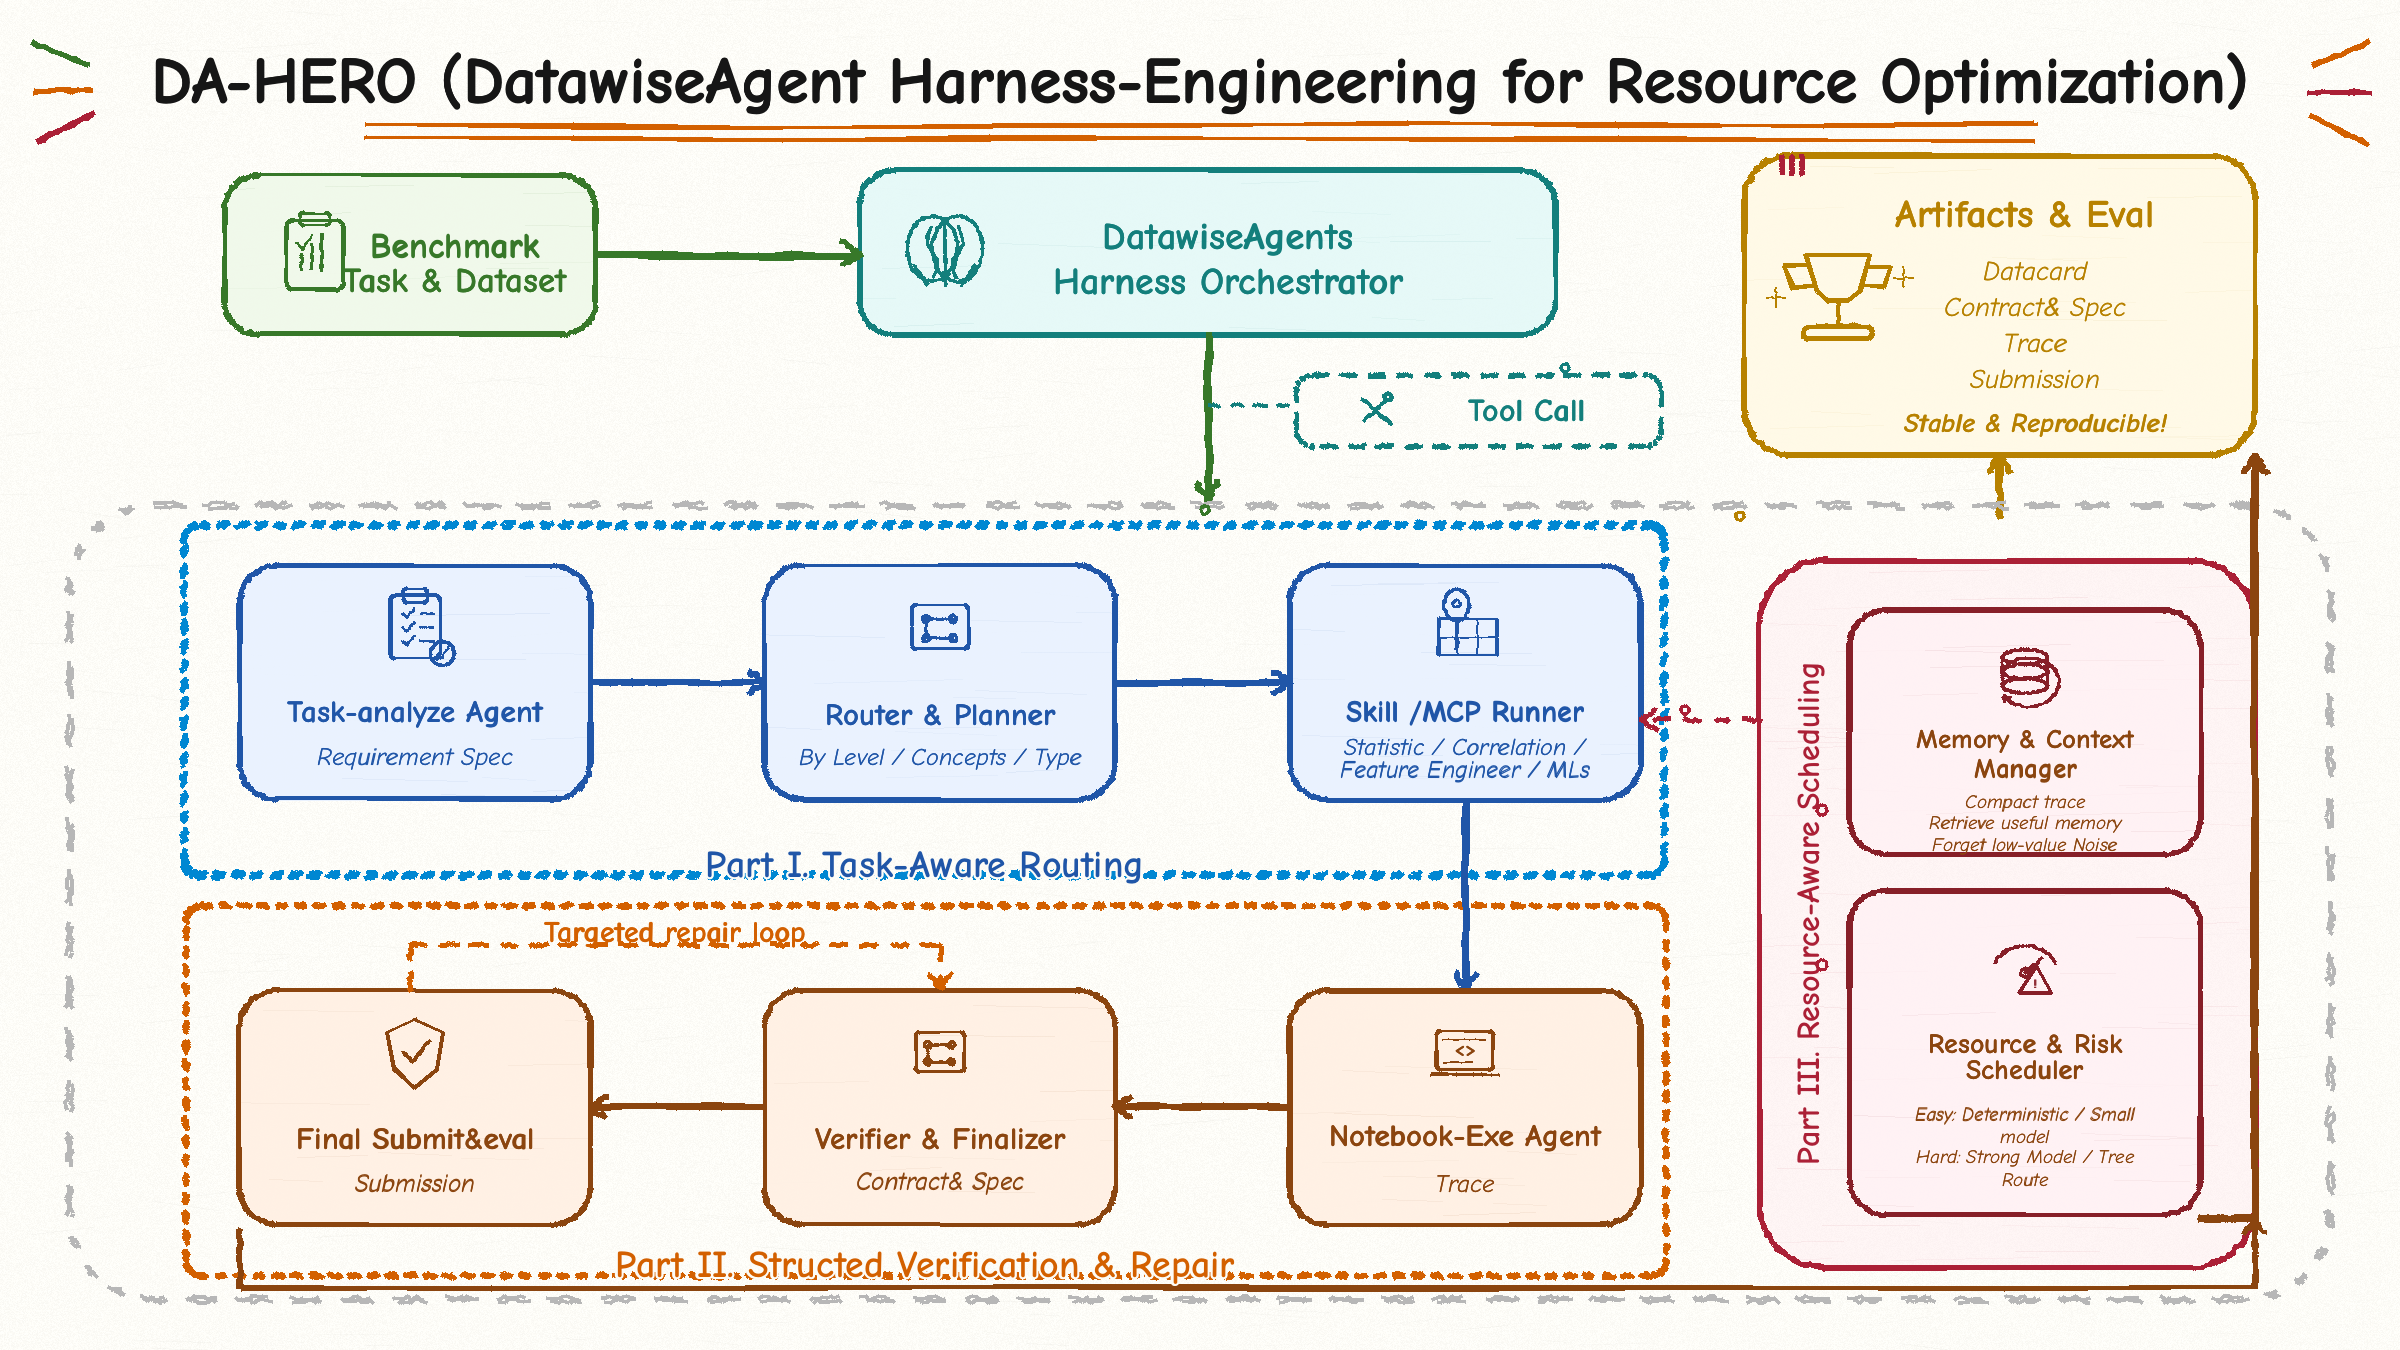
\includegraphics[width=0.96\textwidth]{2404.PNG}
\caption{DA-HERO overview.  The Harness Orchestrator converts benchmark tasks and datasets into requirement specifications, routes them through Task-analyze, Router--Planner, and Skill/MCP modules, executes and repairs notebook traces, and exports DataCards, contracts, traces, and submissions as stable evaluation artifacts.}
\label{fig:da_hero_overview}
\end{figure*}

The \textbf{Answer Spec} specifies the answer name, filtering conditions, grouping variables, statistical method, rounding precision, and forbidden renderings.  The \textbf{Skill Checklist} orders necessary preprocessing and analysis operations by dependency.  The \textbf{Output Contract} gives the deterministic final template.  When benchmark metadata is available, the router is deterministic; otherwise, ambiguity can be delegated to a lightweight model.  Crucially, the Final Block is not LLM-generated.  It extracts a verified value and renders it in the required form, removing format degradation as an independent failure mode.

\subsection{Protocol Adjustments by Task Type}

For \textbf{Summary Statistics}, the harness is maximally prescriptive: column selection, filtering order, aggregation, and rounding are explicitly constrained.  For \textbf{Correlation}, the method must be declared and checked before the value is accepted.  For \textbf{Machine Learning}, the harness shifts from formula enforcement to evidence enforcement: model card, feature treatment, validation strategy, and output semantics.

For \textbf{DataModeling}, the same principle becomes a submission governance problem.  The harness validates schema, row count, ID alignment, probability range, sample-submission consistency, and manifest completeness.  It also flags structurally valid but scientifically weak outputs, such as constant predictions, single-class collapse, global-mean regression, and missing evidence that the final submission improves over a fallback.  This distinction matters: completion is a necessary condition for scoring, but not a proxy for predictive competence.

\subsection{Results on InfiAgentBench}

Table~\ref{tab:task_results} reports the effect of protocol routing.  The harness rerender eliminates format extraction errors and improves all evaluated sub-tasks and difficulty levels.

\begin{table*}[t]
\centering
\caption{Task-aware harness results on InfiAgentBench (Qwen3-32B). Bold indicates best per split.}
\label{tab:task_results}
\begin{tabular}{lcccc}
\toprule
\textbf{Setting} & \textbf{Split} & \textbf{ABQ} & \textbf{PASQ} & \textbf{UASQ} \\
\midrule
Baseline & Medium & 83.72\% & 86.19\% & 86.00\% \\
Harness rerender & Medium & \textbf{91.95\%} & \textbf{93.06\%} & \textbf{93.42\%} \\
\midrule
Baseline & Hard & 66.13\% & 78.49\% & 82.99\% \\
Harness rerender & Hard & \textbf{78.41\%} & \textbf{84.75\%} & \textbf{87.19\%} \\
\bottomrule
\end{tabular}
\end{table*}

\begin{figure*}[t]
\centering
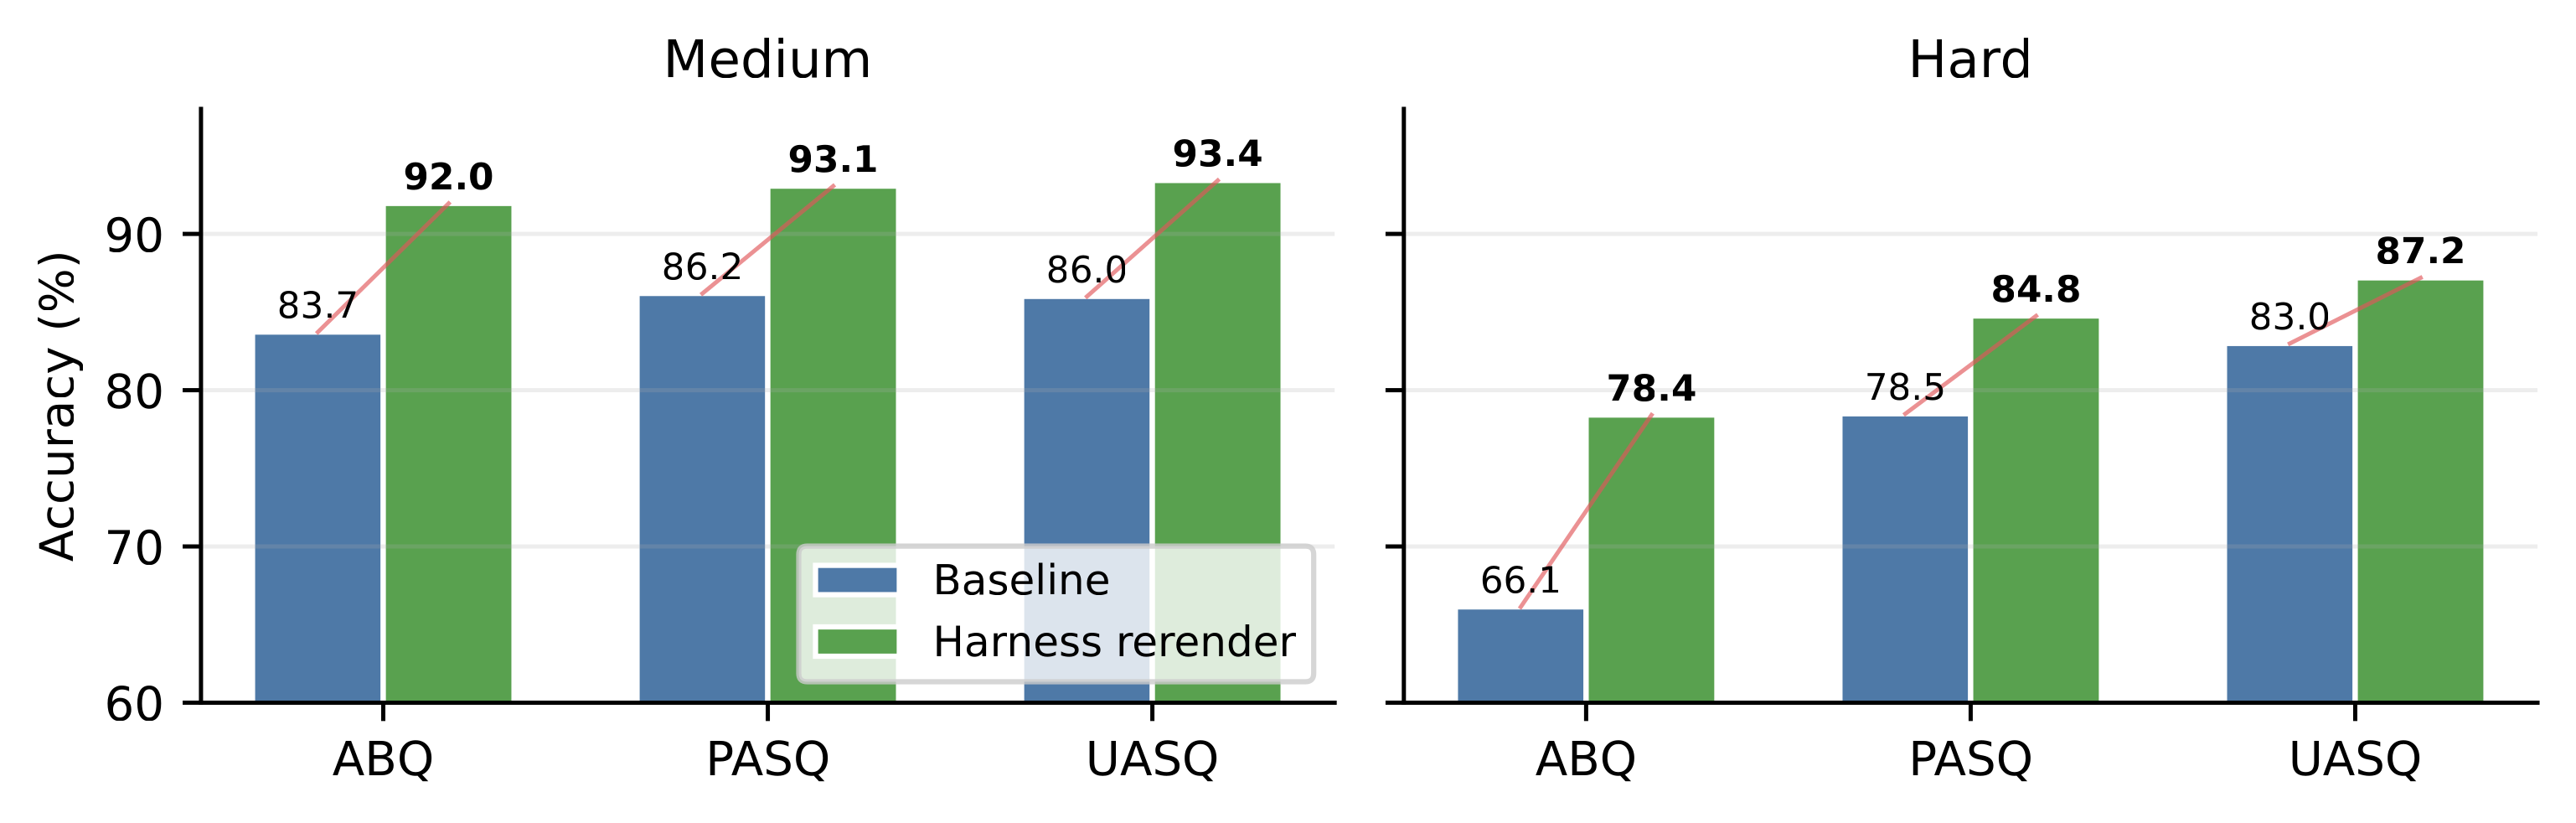
\includegraphics[width=0.86\textwidth]{task_harness_results.png}
\caption{Task-aware harness gains by split and sub-task.  The largest absolute gain appears on Hard ABQ, where answer specification, verification, and deterministic final rendering prevent otherwise silent definition and format errors.}
\label{fig:task_harness_results}
\end{figure*}

Medium ABQ improves by 8.23pp, showing that many apparent reasoning failures are actually failures of specification and rendering.  PASQ and UASQ also improve, indicating that protocol routing stabilizes statistical definitions beyond answer formatting.  On Hard ABQ, the 12.28pp gain is the largest, but the average number of execution branches rises from 1.0 to 2.97.  Protocols therefore create useful search pressure; Section~\ref{sec:resource} addresses how to fund that search without letting cost expand unchecked.

\subsection{Results on DataModeling}

On DataModeling, Qwen3.5-35B-A3B achieves 73/74 completion with a normalized performance score of 0.5318 and an average time of 288.6 seconds, outperforming the Qwen2.5 baseline (68/74, 0.4290, 760.3s).  Yet Qwen3-VL variants reach 74/74 structural completion while scoring only 0.3127 and 0.2873.  This exposes a \textbf{completion--performance gap}: a scoreable CSV can still encode weak modeling.  Representative re-tests sharpen the point.  8B Titanic (0.7877 AUC) and 32B Santander (0.8116 AUC) produce meaningful predictions on well-structured tabular tasks, but both require manifest repair and struggle when task success depends on domain-specific modeling strategy.  The DataModeling harness therefore treats submission validity as the floor and modeling evidence as the object of governance.

\section{Structured Time-for-Performance}
\label{sec:structured}

\subsection{Why Unstructured Interaction Fails}

Notebook agents often rely on an implicit assumption: if a model can interact longer with an environment, it should eventually improve.  Our traces show a more complicated reality.  Longer histories can preserve useful computation, but they also preserve stale variables, failed branches, verbose debug output, and earlier wrong answers.  The agent may compute a correct statistic in one cell, debug an unrelated issue later, and then overwrite the final answer with a transient intermediate.  Additional interaction becomes productive only when it is organized around verifiable state.

We observe three recurring pathologies.  \textbf{Context contamination} occurs when irrelevant notebook state re-enters the final reasoning step.  \textbf{Non-monotonic verification} occurs when a heavy semantic oracle over-constrains a correct but differently expressed answer.  \textbf{Branch proliferation} occurs when search produces multiple candidates without a principled selection criterion.  The problem is not interaction itself; the problem is interaction without typed artifacts.

\subsection{Verifiable Artifact Pipeline}

DA-HERO decomposes interaction into six artifacts, each checkable before the next stage consumes it:

\begin{enumerate}
    \item \textbf{DataCard}: a deterministic profile of columns, types, missingness, and numeric ranges, computed once per dataset.
    \item \textbf{Answer Spec}: a structured representation of answer name, required columns, filters, aggregation, precision, and output format.
    \item \textbf{Skill Checklist}: a dependency-ordered set of preprocessing and analysis steps derived from the DataCard and Answer Spec.
    \item \textbf{Notebook Execution}: code generation and execution constrained by the preceding artifacts.
    \item \textbf{Verifier}: a structural and semantic check that reports the violated constraint and observed state.
    \item \textbf{Final Block}: a deterministic renderer that emits the verified answer in the required format.
\end{enumerate}

The critical mechanism is targeted retry.  When verification fails, the model receives the violated constraint and relevant intermediate output, not the full notebook transcript.  Retry contexts are typically under 500 tokens rather than thousands of tokens of historical state.  This converts retry from conversational persistence into localized repair.

\begin{figure*}[t]
\centering
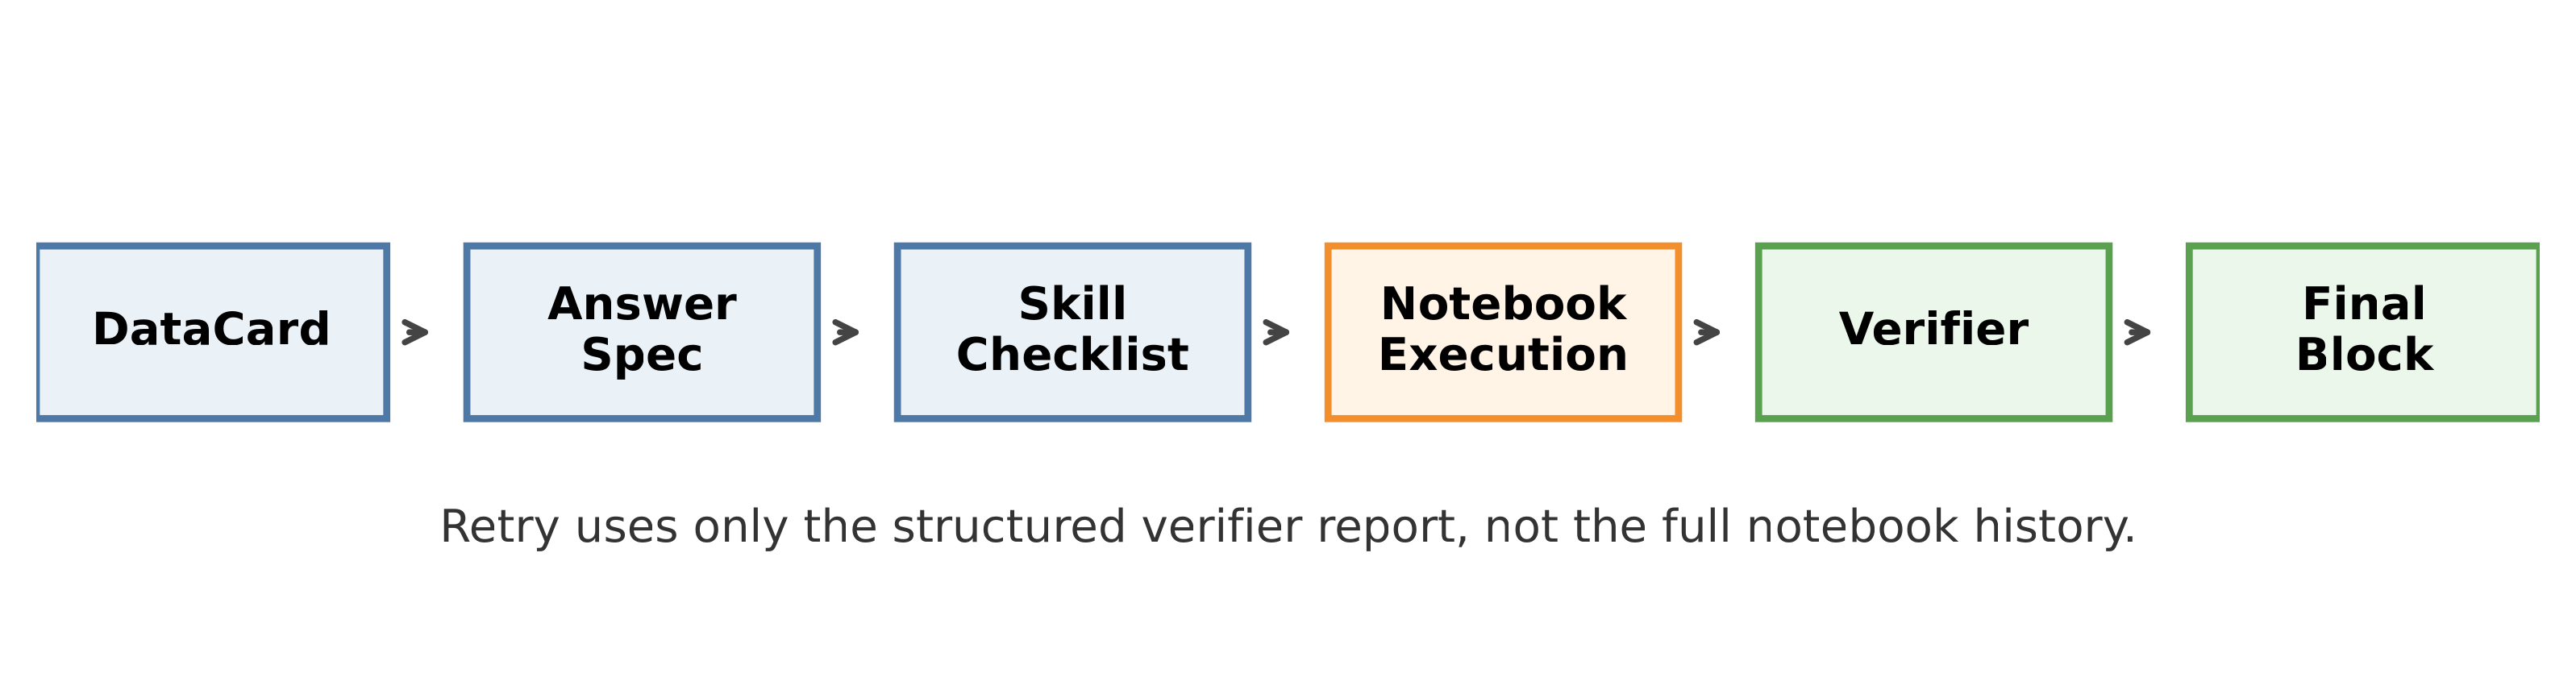
\includegraphics[width=0.9\textwidth]{artifact_pipeline.png}
\caption{Verifiable artifact pipeline. Each stage emits a compact artifact that can be checked before the next stage consumes it. Repair is conditioned on the structured verifier report rather than the full notebook history.}
\label{fig:artifact_pipeline}
\end{figure*}

\subsection{Lightweight and Full Verification Regimes}

We instantiate two regimes.  \textbf{\texttt{harness\_light}} enables DataCard, Answer Spec, Skill Checklist, deterministic formatting, and programmatic finalization.  It avoids semantic oracle calls and multi-branch search.  \textbf{\texttt{harness\_full}} adds semantic verification, targeted retry, and optional multi-branch execution for hard questions.  The distinction is not model size; it is the amount of governance applied to the same model.

\subsection{Results}

Table~\ref{tab:structured_results} compares the regimes against a baseline with only the original post-hoc reformatting mechanism.  We use Qwen3.5-Flash to test whether structure can compensate for weaker reasoning.

\begin{table*}[t]
\centering
\caption{Structured interaction results (Qwen3.5-Flash, InfiAgentBench small-set).}
\label{tab:structured_results}
\begin{tabular}{lccc}
\toprule
\textbf{Setting} & \textbf{ABQ} & \textbf{Hard ABQ} & \textbf{Avg Runtime (s)} \\
\midrule
Baseline + original reformat & 48.94\% & 44.00\% & 30.24 \\
\texttt{harness\_light} & 51.57\% & 47.32\% & 37.03 \\
\texttt{harness\_full} & 52.83\% & 49.44\% & 43.79 \\
\bottomrule
\end{tabular}
\end{table*}

\begin{figure*}[t]
\centering
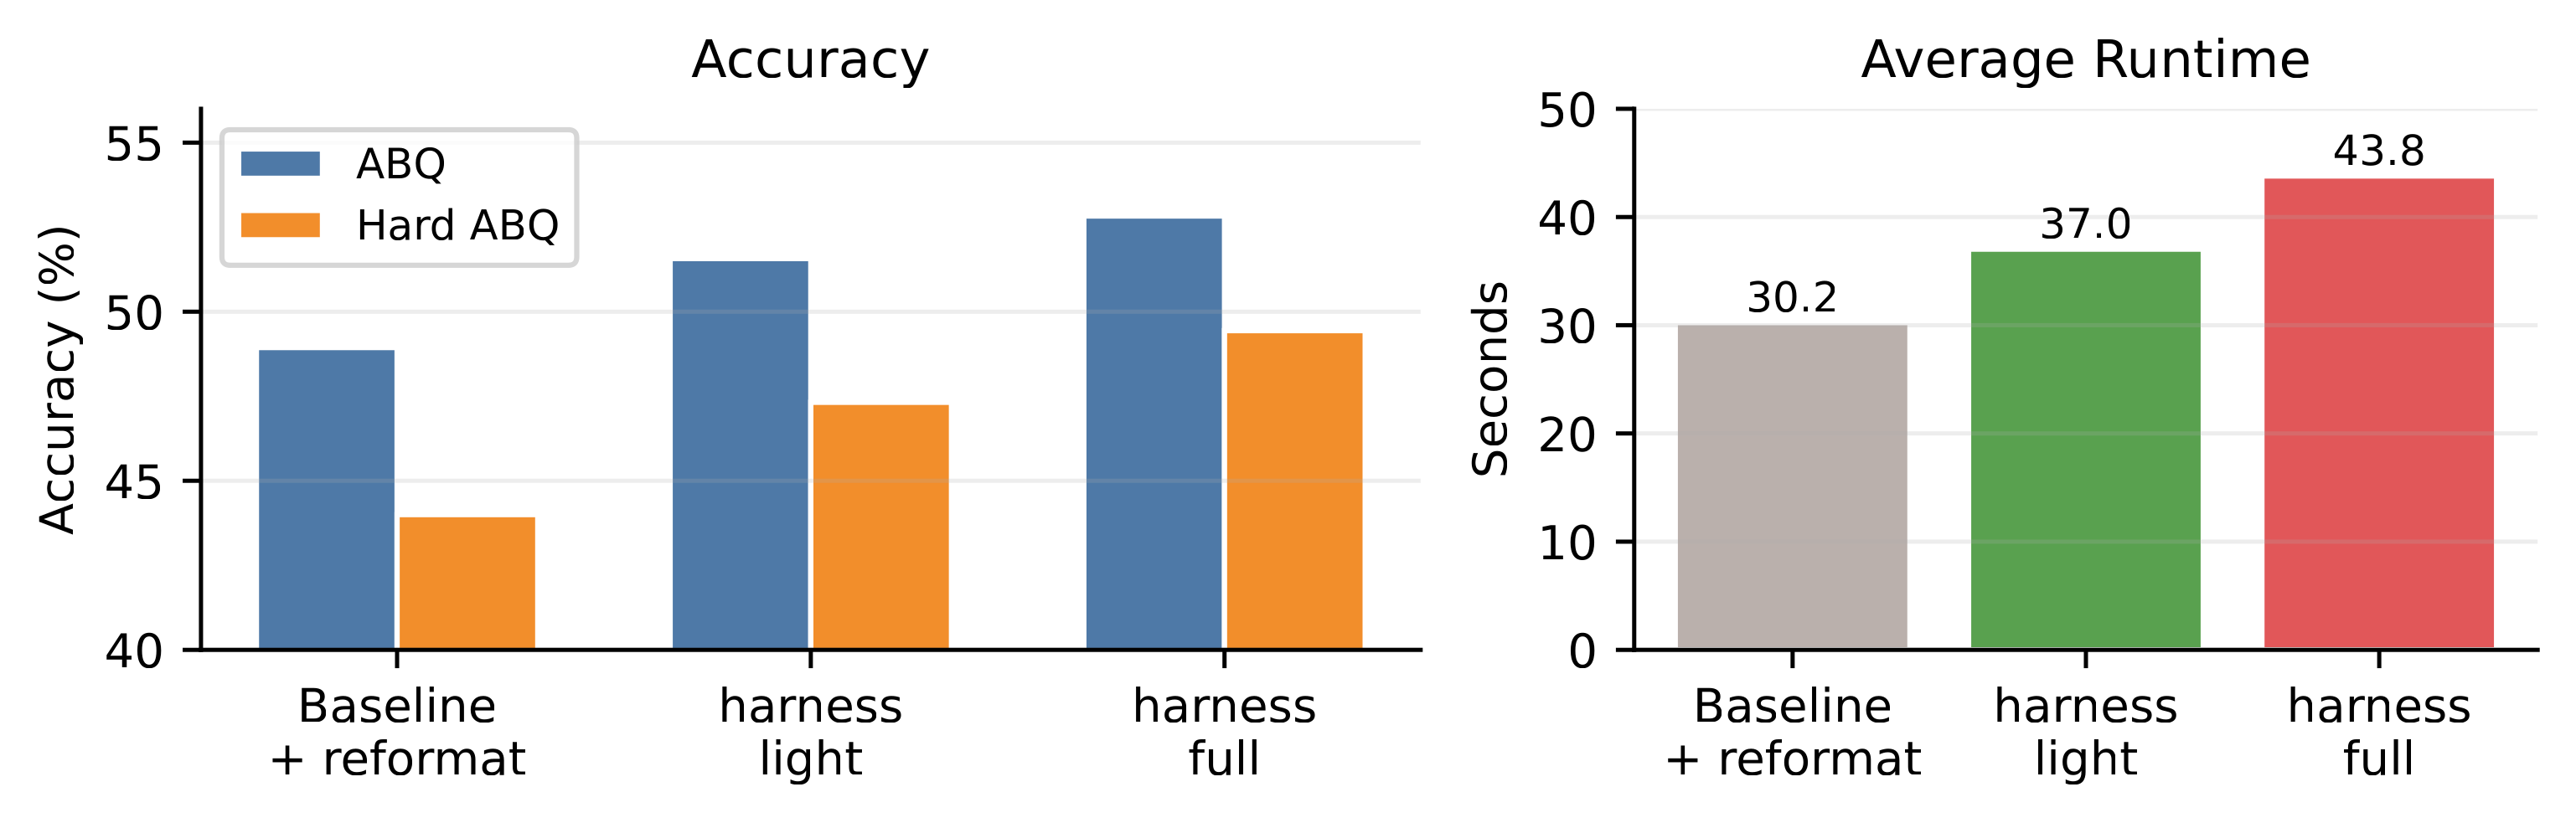
\includegraphics[width=0.86\textwidth]{structured_results.png}
\caption{Structured interaction on the Qwen3.5-Flash small-set experiment. Lightweight structure improves accuracy with modest overhead, while full verification provides additional gains on harder questions at higher runtime.}
\label{fig:structured_results}
\end{figure*}

Both structured regimes outperform the baseline.  \texttt{harness\_light} improves ABQ by 2.63pp and Hard ABQ by 3.32pp with modest overhead.  \texttt{harness\_full} adds 1.26pp ABQ and 2.12pp Hard ABQ at additional cost.  The result argues against a universal ``more harness'' rule: lightweight structure is enough for many easy and medium tasks, while full verification is valuable when semantic ambiguity is likely.  This observation motivates risk-based dispatch.

\subsection{Artifact Reuse and Communication Efficiency}

Artifacts also serve as compact communication channels.  A DataCard is reused across questions sharing a dataset; an Answer Spec compresses a natural-language request into a typed contract; a Verifier report replaces full transcript retransmission.  In our experiments, artifact reuse reduces average tokens per question by approximately 30\% relative to repeatedly re-reading and re-describing the dataset.  The performance gain is therefore paired with a communication gain: the agent receives less text, but more useful state.

\section{Resource-Aware Scheduling}
\label{sec:resource}

\subsection{The EqTok Metric}

A governed agent should be evaluated not only by accuracy, but by the price of the reasoning used to obtain it.  Raw token count is inadequate because different model tiers have different prices; API-call count is also inadequate because many cheap calls may cost less than a single large-model call.  We define \textbf{EqTok} (Equivalent Tokens) as a pricing-weighted token count:

\begin{equation}
\mathrm{EqTok} = T_{32B} + 0.5 \cdot T_{14B} + 0.25 \cdot T_{8B}
\label{eq:eqtok}
\end{equation}

where $T_M$ is the output-token consumption of model tier $M$.  The coefficients reflect the approximate Qwen API pricing ratios on our deployment platform, normalized to 32B-equivalent units.  EqTok is intentionally family-specific: other providers require recalibration.  Its purpose is to compare mixed-model pipelines under a single economic unit.

\subsection{Risk-Stratified Sub-Task Routing}

DA-HERO decomposes execution into sub-tasks and assigns each to the lowest-cost processing tier consistent with acceptable error risk.  Deterministic stages such as profiling, cleanup, verification, and final formatting do not call an LLM.  Low-risk reasoning uses smaller models; high-risk code generation and complex debugging are routed to stronger models.

\begin{table*}[t]
\centering
\caption{Risk-stratified sub-task routing. Each sub-task is assigned to the lowest-cost processing tier consistent with acceptable error risk.}
\label{tab:risk_routing}
\footnotesize
\begin{tabular}{p{0.22\textwidth}p{0.38\textwidth}p{0.28\textwidth}}
\toprule
\textbf{Sub-Task} & \textbf{Description} & \textbf{Tier} \\
\midrule
Data Profiling & Read schema, types, missing values, ranges & Deterministic \\
Answer Spec Parsing & Extract answer name, columns, format & Rule-first; 8B/14B fallback \\
Task Routing & Classify concept, difficulty, risk level & Rule-first; 8B/14B fallback \\
Step Planning & Decompose question into analysis steps & 8B (easy), 14B (med), 32B (hard) \\
Code Generation & Write data processing / ML code & 14B (easy), 32B (med/hard) \\
Debugging & Fix runtime and logic errors & 8B/14B (simple), 32B (complex) \\
Post-Debug Cleanup & Remove error cells, keep working path & Deterministic \\
Verification & Check constraints against Answer Spec & Deterministic \\
Final Formatting & Render into required output format & Deterministic \\
\bottomrule
\end{tabular}
\end{table*}

The scheduler is risk-proportional rather than model-centric.  It asks which stage can damage the final answer if it fails, not which model is globally preferred.  This distinction is essential: strong models can be cheaper end-to-end when they avoid repeated debugging, while small models can be wasteful when routed into stages beyond their competence.

\subsection{Dialogue Reduction Mechanisms}

We reduce LLM calls through five mechanisms:

\begin{enumerate}
    \item \textbf{Deterministic Artifacts}: DataCard, unambiguous Answer Spec parsing, and Final Block are computed programmatically.
    \item \textbf{Spec-to-Plan Generation}: Structured Answer Specs generate operation plans through templates rather than free-form exploration.
    \item \textbf{One-Shot Execution}: Low-risk questions execute with pre-filled artifacts in a single model call.
    \item \textbf{Verifier-Triggered Retry}: Repair is activated only by a structured failure report.
    \item \textbf{Cross-Question Artifact Reuse}: Shared datasets reuse profiling and normalization artifacts across questions.
\end{enumerate}

\subsection{Resource Ablation Results}

Table~\ref{tab:resource_results} compares a 32B single-model baseline, a Small Model Rules configuration, and a configuration that additionally enables dialogue reduction.

\begin{table*}[t]
\centering
\caption{Resource ablation results on InfiAgentBench. EqTok is reported in millions of 32B-equivalent tokens.}
\label{tab:resource_results}
\begin{tabular}{lccc}
\toprule
\textbf{Configuration} & \textbf{ABQ} & \textbf{EqTok (M)} & \textbf{API Calls} \\
\midrule
32B baseline & 81.74\% & 5.960 & 1,621 \\
Small Model Rules & 78.42\% & 3.517 & 1,956 \\
+ Dialogue Reduction & 78.63\% & 3.298 & 1,874 \\
\bottomrule
\end{tabular}
\end{table*}

\begin{figure*}[t]
\centering
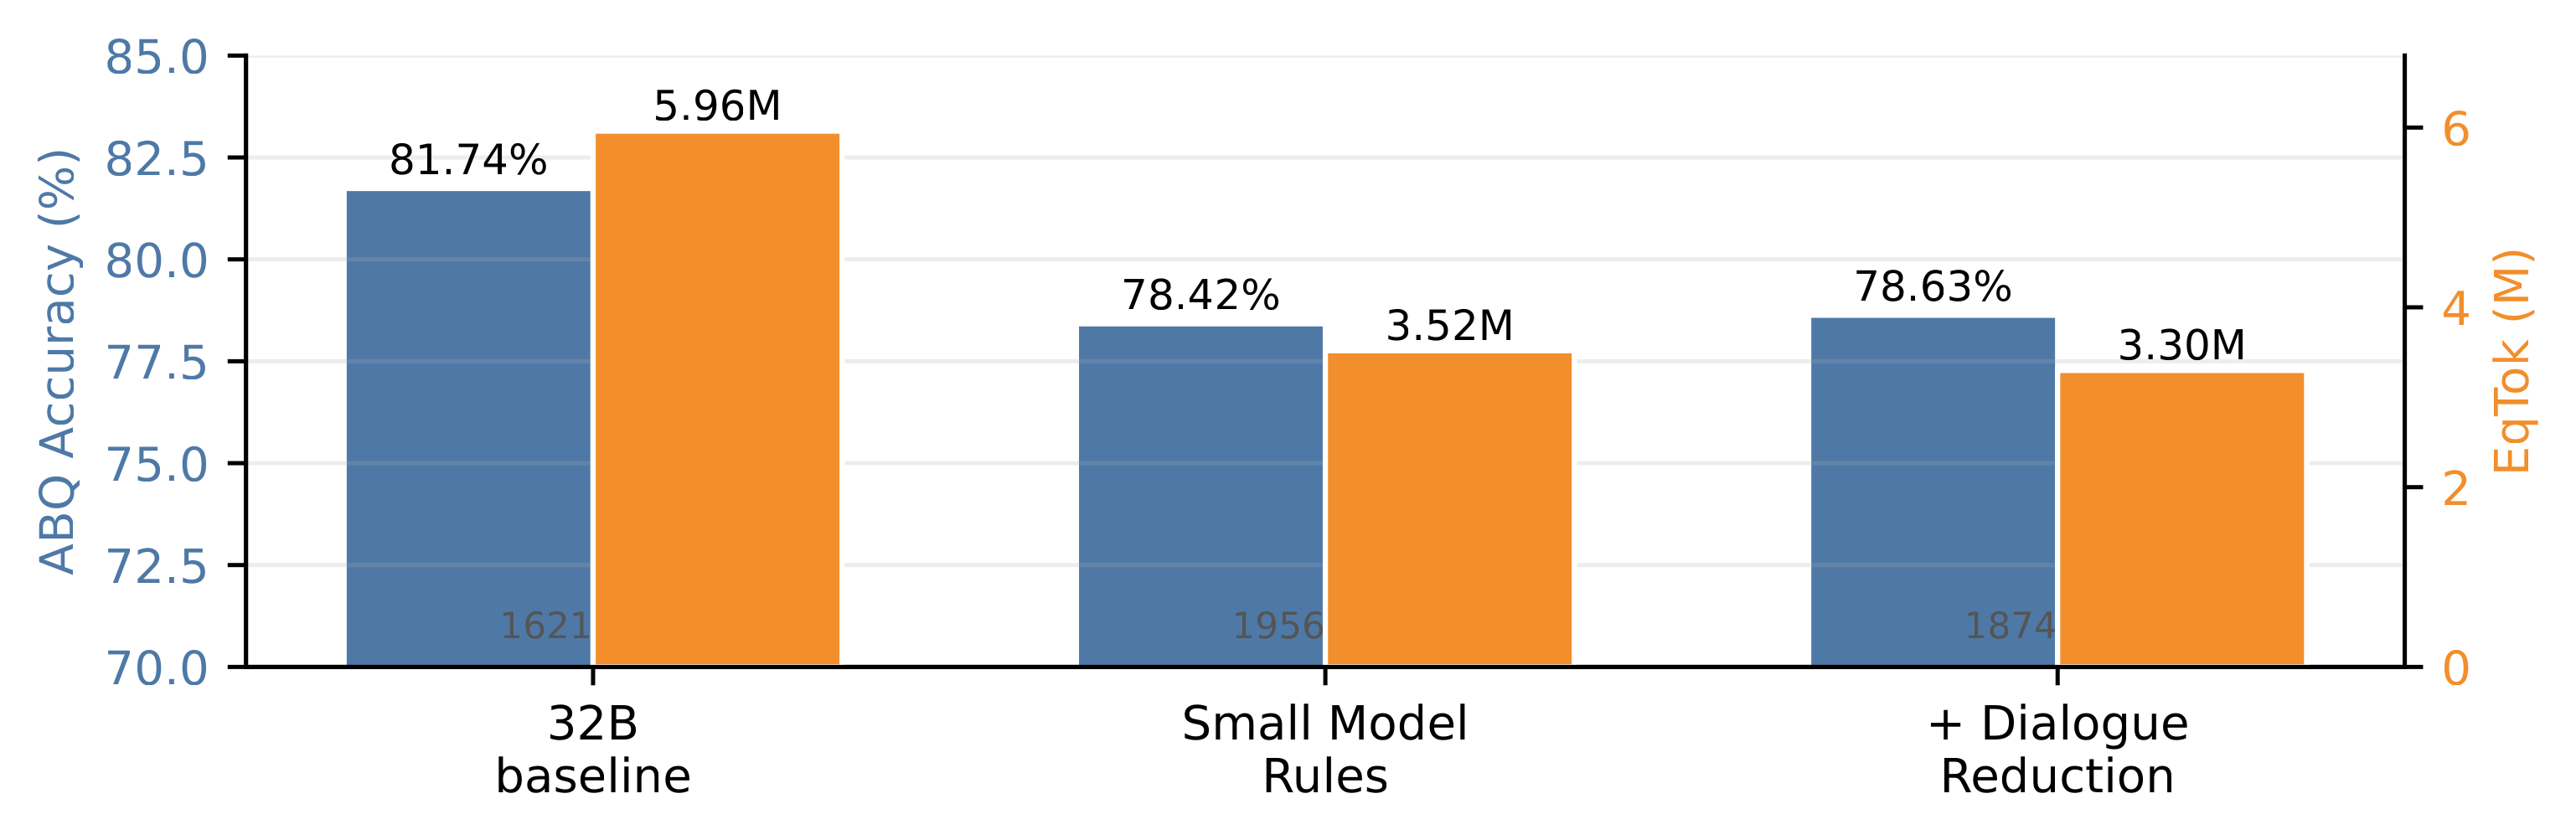
\includegraphics[width=0.86\textwidth]{resource_ablation.png}
\caption{Resource ablation with pricing-normalized EqTok. Smaller-model routing increases the number of API calls but sharply reduces 32B-equivalent token cost, retaining most baseline ABQ accuracy.}
\label{fig:resource_ablation}
\end{figure*}

Small Model Rules reduces EqTok by 41.0\% while retaining 95.9\% of baseline accuracy.  Dialogue reduction lowers EqTok further to 3.30M, a 44.7\% total reduction, with a small accuracy gain.  The call count rises in the smaller-model settings, but EqTok exposes the real economics: more calls can still be cheaper when they are routed through low-cost tiers.  The result supports our scheduling thesis: resource efficiency comes from matching model strength to stage risk, not from uniformly shrinking or uniformly enlarging the model.

\section{Integrated Architecture}
\label{sec:integration}

Figure~\ref{fig:architecture} illustrates the integrated DA-HERO architecture as a separation between a governance plane and an execution plane.  The governance plane contains the Harness Orchestrator, task-aware routing, memory/context management, and resource-risk scheduling.  The execution plane contains the notebook-execution agent, verifier/finalizer, targeted repair loop, and final submission path.  Each stage is governed by two decisions: what protocol constrains the stage, and what processing tier is justified by its risk.

\begin{figure*}[t]
\centering
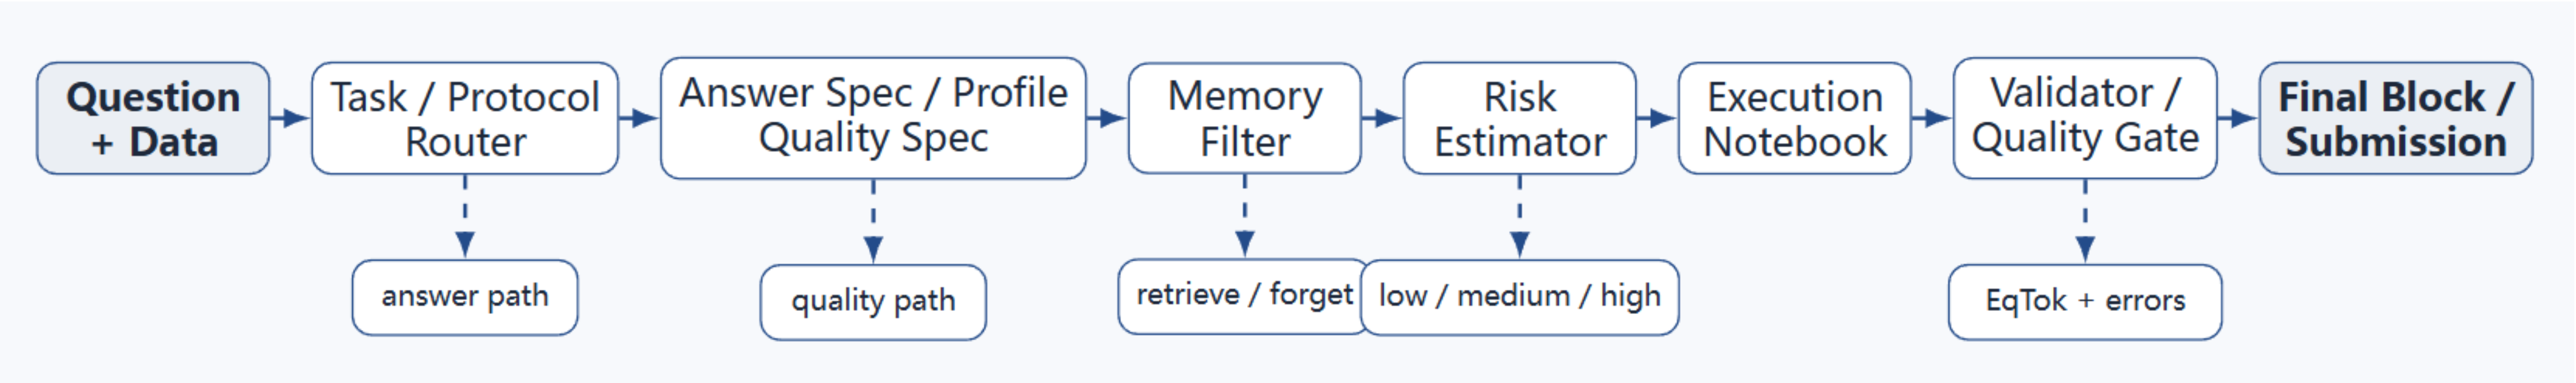
\includegraphics[width=0.9\textwidth]{fig1.png}
\caption{Integrated DA-HERO architecture.  A Harness Orchestrator coordinates task-aware routing, Skill/MCP execution, structured verification and repair, memory/context filtering, resource-risk scheduling, and artifact-based evaluation.  The system separates the governance plane from notebook execution while preserving reproducible DataCard, contract, trace, and submission artifacts.}
\label{fig:architecture}
\end{figure*}

The architecture operationalizes three principles:

\begin{enumerate}
    \item \textbf{Task semantics precede execution}: The agent should not write code before the task has been represented as a protocol.  Closed-form analysis, predictive modeling, correlation, and multi-concept ML require different constraints.
    \item \textbf{Evidence travels in artifacts}: The system passes DataCards, Answer Specs, Verifier reports, and manifests rather than raw conversation logs.  This preserves high-value state and removes irrelevant notebook debris.
    \item \textbf{Compute follows risk}: Deterministic programs handle no-risk stages; lightweight models handle low-risk ambiguity; strong models are reserved for stages where reasoning errors propagate to the final answer.
\end{enumerate}

This integrated view also clarifies the DataModeling result.  Structural completion is not equivalent to predictive performance.  Qwen3-VL can complete every task structurally while still producing low-information submissions.  A quality gate detects this gap; a governed modeling protocol narrows it; but closing it entirely requires stronger modeling competence.  DA-HERO therefore separates what the runtime can govern from what the base model must still learn.

\section{Discussion and Boundary Analysis}
\label{sec:discussion}

\subsection{Where Harness Governance Ends}

DA-HERO improves the conditions under which an agent reasons, but it does not erase the need for model competence.  The boundary is visible in three regimes.

\textbf{Multi-concept hard questions} require simultaneous reasoning about preprocessing, feature construction, model choice, validation, and final reporting.  Harness protocols can prevent answer-name drift and format collapse, but they cannot make an incorrect modeling strategy correct.

\textbf{Predictive modeling gaps} show the same boundary at larger scale.  A quality gate can detect constant predictions, single-class collapse, missing manifests, and invalid probability ranges.  It can also route the agent back toward repair.  But when success depends on domain-specific feature engineering, text modeling, grouped validation, or time-aware splitting, the base model's data-science competence remains decisive.

\textbf{Memory saturation} is a runtime boundary.  Retaining everything is not a memory strategy; it is an invitation for stale state to compete with useful evidence.  Our artifact-based design points toward selective memory: keep typed, recent, high-impact artifacts; discard raw interaction traces once their useful information has been compiled.

\subsection{Design Principles}

The experiments yield five design principles for reliable and economical data-science agents:

\begin{enumerate}
    \item \textbf{Classify before constraining}: choose the harness protocol from task semantics rather than applying one universal prompt.
    \item \textbf{Verify at artifact boundaries}: validate each typed artifact before the next stage consumes it; repair from the failure report, not the full transcript.
    \item \textbf{Separate completion from competence}: a valid file or parseable answer is only the outer shell; modeling evidence determines whether the result is scientifically meaningful.
    \item \textbf{Route compute by risk}: reserve large models for stages where reasoning errors are expensive; use deterministic programs and smaller models elsewhere.
    \item \textbf{Measure cost in the unit that matters}: evaluate mixed-model agents with pricing-normalized EqTok rather than raw tokens or API calls.
\end{enumerate}

\subsection{Limitations and Future Work}

Our resource coefficients are calibrated to the Qwen deployment used in this study and should be recalibrated for other model families.  The task router benefits from benchmark metadata; production systems will need stronger automatic difficulty and concept estimators.  The memory component remains intentionally lightweight and should be extended with empirically calibrated importance and recency policies.  Finally, the DataModeling completion--performance gap indicates a natural next step: combine runtime governance with targeted model improvement, such as fine-tuning or tool-augmented modeling specialists for tasks where general-purpose agents consistently underperform.

\section{Conclusion}

We presented DA-HERO, a governed runtime for data-science agents that treats harness design as a first-class mechanism for reliability, performance, and cost control.  The system protocolizes task semantics, converts long interactions into verifiable artifacts, and routes computation according to stage risk.  On InfiAgentBench, protocol routing eliminates format-level extraction errors and yields large gains on Medium and Hard ABQ.  Structured artifacts improve weak-model performance by turning retry into localized repair.  Risk-stratified scheduling reduces EqTok by roughly 40\% while preserving most baseline accuracy.  On DataModeling, the analysis exposes a sharper distinction between structural completion and predictive competence, motivating quality gates and modeling evidence rather than submission validity alone.  The broader lesson is that the next generation of data-science agents should be built less like unconstrained notebook chatbots and more like governed scientific workflow systems: protocolized before execution, evidence-bearing during execution, and risk-aware in the way they spend computation.

\bibliography{datawiseagent_refs}

\end{document}
